\documentclass[10pt,twoside]{article}
\usepackage[ngerman]{babel}
\usepackage[utf8]{inputenc}
\usepackage{textcomp,gensymb}
\usepackage{longtable}
\usepackage{lscape}
%\usepackage[latin1]{inputenc}
\usepackage{amsmath,thmtools}
\usepackage{siunitx}
\usepackage{enumitem} 
\usepackage{array}
\usepackage{amstext}
\usepackage{amssymb}
\usepackage{stmaryrd}
\usepackage{verbatim}
\usepackage{mathrsfs}
\usepackage{extarrows}
\usepackage[arrow, matrix, curve]{xy}
\usepackage[centering,includeheadfoot,top=25mm, left=40mm, right=25mm, bottom=30mm]{geometry}
\usepackage{gensymb}
\usepackage{graphicx}
\usepackage{framed}
\usepackage[usenames,dvipsnames]{xcolor}
\usepackage{float}
\usepackage{sidecap}
\usepackage{tikz,lipsum,lmodern}
\usepackage{import}
\usepackage{fancyhdr}
\usepackage{fancybox}
\usepackage{caption}
\usepackage{subcaption}
\usepackage{esint}
\parskip 10pt
\parindent 0pt
\DeclareGraphicsRule{.tif}{png}{.png}{`convert #1 `basename #1 .tif`.png} 
\makeindex
\usepackage[colorlinks,pdfpagelabels,pdfstartview = FitH,bookmarksopen = true,bookmarksnumbered = true,linkcolor = black,plainpages =false,hypertexnames = false,citecolor = black] {hyperref}
\makeatletter
\def\@tocline#1#2#3#4#5#6#7{\relax
  \ifnum #1>\c@tocdepth % then omit
  \else
    \par \addpenalty\@secpenalty\addvspace{#2}%
    \begingroup \hyphenpenalty\@M
    \@ifempty{#4}{%
      \@tempdima\csname r@tocindent\number#1\endcsname\relax
    }{%
      \@tempdima#4\relax
    }%
    \parindent\z@ \leftskip#3\relax \advance\leftskip\@tempdima\relax
    \rightskip\@pnumwidth plus4em \parfillskip-\@pnumwidth
    #5\leavevmode\hskip-\@tempdima
      \ifcase #1
       \or\or \hskip 1em \or \hskip 2em \else \hskip 3em \fi%
      #6\nobreak\relax
    \dotfill\hbox to\@pnumwidth{\@tocpagenum{#7}}\par
    \nobreak
    \endgroup
  \fi}
  \setcounter{tocdepth}{3}
\makeatother
%%%%%%%%%%%%%%%%%%%%%%%RedeclareMathOperator
\makeatletter
\newcommand\RedeclareMathOperator{%
  \@ifstar{\def\rmo@s{m}\rmo@redeclare}{\def\rmo@s{o}\rmo@redeclare}%
}
% this is taken from \renew@command
\newcommand\rmo@redeclare[2]{%
  \begingroup \escapechar\m@ne\xdef\@gtempa{{\string#1}}\endgroup
  \expandafter\@ifundefined\@gtempa
     {\@latex@error{\noexpand#1undefined}\@ehc}%
     \relax
  \expandafter\rmo@declmathop\rmo@s{#1}{#2}}
% This is just \@declmathop without \@ifdefinable
\newcommand\rmo@declmathop[3]{%
  \DeclareRobustCommand{#2}{\qopname\newmcodes@#1{#3}}%
}
\@onlypreamble\RedeclareMathOperator
\makeatother
\renewcommand{\sectionmark}[1]{\markboth{#1}{}}
\lhead{\fancyplain{}{\textit{\leftmark}}}
%%%%%%%%%%%%%%%%%%%%%%%%%%%%%%%%%%%%%%%%%%%%%%%%%%%%%%%%%%%%%%%%%%%%%%%%%%%%%%%%%%Bestimmte Mengen
\newcommand{\C}{\ensuremath{\mathbb{C}}}
\newcommand{\F}{\ensuremath{\mathbb{F}}}
\renewcommand{\P}{\ensuremath{\mathbb{P}}}
\newcommand{\R}{\ensuremath{\mathbb{R}}}
\newcommand{\N}{\ensuremath{\mathbb{N}}}
\newcommand{\Q}{\ensuremath{\mathbb{Q}}}
\newcommand{\Z}{\ensuremath{\mathbb{Z}}}
%%%%%%%%%%%%%%%%%%%%%%%%%%%%%%%%%%%%%%%%%%%%%%%%%%%%%%%%%%%%%%%%%%%%%%%%%%%%%%%%%%Pfeile
\newcommand{\imp}{\Longrightarrow}
\newcommand{\pim}{\Longleftarrow}
\newcommand{\nach}{\longrightarrow}
\newcommand{\hcan}{\longleftarrow}
\newcommand{\nachmenge}{\longmapsto}
\newcommand{\aq}{\Longleftrightarrow}
\newcommand{\surj}{\twoheadrightarrow}
\newcommand{\jrus}{\twoheadleftarrow}
\newcommand{\inj}{\hookrightarrow}
\newcommand{\jni}{\hookleftarrow}
\newcommand{\ximp}{\xLongrightarrow}			%  \xLongrightarrow[\text{unten Text}]{\text{oben Text}} 
																		%%%% Implikation Text oben und untern 
\newcommand{\xpim}{\xLongleftarrow}
\newcommand{\xaq}{\xLeftrightarrow}			%  \xLeftrightarrow[\text{unten Text}]{\text{oben Text}} 
																		%%%% Äquivalenz Text oben und unten
\newcommand{\xnach}{\xlongrightarrow}		
\newcommand{\xhcan}{\xlongleftarrow}										

\renewcommand{\l}{\left\vert}   						%linker Betragsstrich
\renewcommand{\r}{\right\vert}						%rechter Betragsstrich
\newcommand{\ecap}{\cap \ldots \cap}			%Schnit ... Schnitt
\newcommand{\ecup}{\cup \ldots \cup}			%Vereinigung ... Vereinigung
\newcommand{\eplus}{+ \ldots +}					% + ... +
\newcommand{\ekomma}{{,} \ldots {,}}			% , ... ,
\newcommand{\x}{\times}								%  kreuz 
\renewcommand{\d}{~\text{d}}
\renewcommand{\tilde}{\widetilde}
\DeclareMathOperator{\rot}{\text{rot}}
\RedeclareMathOperator{\div}{\text{div}}
\DeclareMathOperator{\laplace}{\vartriangle}
\renewcommand{\epsilon}{\varepsilon}
\newcommand{\qed}{\hfill$\square$\par}
\renewcommand{\bar}{\overline}
%%%%%%%%%%%%%%%%%%%%%%%%%%%%%%%%%%%%%%%%%%%%%%%%%%%%%%%%%%%%%%%%%%%%%%%%%%%%%%%%%%  Hoch minus Zahl
\renewcommand{\1}{^{-1}}				
\renewcommand{\2}{^{-2}}
\newcommand{\3}{^{-3}}
\newcommand{\4}{^{-4}}
\newcommand{\5}{^{-5}}
\newcommand{\6}{^{-6}}
\newcommand{\7}{^{-7}}
\newcommand{\8}{^{-8}}
\newcommand{\9}{^{-9}}
%%%%%%%%%%%%%%%%%%%%%%%%%%%%%%%%%%%%%%%%%%%%%%%%%%%%%%%%%%%%%%%%%%%%%%%%%%%%%%%%%% Definitionsgleich
\newcommand{\define}{\ensuremath{\mathrel{\mathop:}=}} % hübscheres :=, da = zentriert wird relativ zu :
\newcommand{\enifed}{\ensuremath{=\mathrel{\mathop:}}} % hübscheres =:, da = zentriert wird relativ zu :
%%%%%%%%%%%%%%%%%%%%%%%%%%%%%%%%%%%%%%%%%%%%%%%%%%%%%%%%%%%%%%%%%%%%%%%%%%%%%%%%%%Box
\usepackage[most]{tcolorbox}
\definecolor{myColor}{rgb}{0.9,0.9,0.9}		% Farbe für Hintergrund
\definecolor{mycolor}{HTML}{9FB6CD}			% Farbe für Überschriftframe
%%%%%%%%%%%%%%%%%%%%%%%%%%%%%%%%%%%%%%%%%%%%%%%%%%%%%%%%%%%%%%%%%%%%%%%%%%%%%%%%%Abstände
%\, = ein sehr kleiner Abstand
%~ =Leertaste
%\enspace = so breit wie eine Ziffer
%\quad = so breit, wie ein Buchstabe hoch ist
%\qquad = dobbelt so breit wie ein \quad
%\hfill = ein Abstand, der sich von 0 bis unendlich ausdehnen kann
%\hspace{x.ycm} = ein Abstand, der x,y cm lang ist
%%%%%%%%%%%%%%%%%%%%%%%%%%%%%%%%%%%%%%%%%%%%%%%%%%%%%%%%%%%%%%%%%%%%%%%%%%%%%%%%%%XY-Pics
%\begin{figure}[H]
%\begin{center}                     
%\begin{equation*}
%\mbox{%
%$%{\xymatrix{
%
%}
%}$
%}
%\end{equation*}
% \end{center}
% \end{figure}

%\xymatrix{}
%	A  \ar@{.>}[]^"funktion"  B  					gepunkteter Pfeil nach rechts [r] nach links [l]
%	B  \ar2@{<->}[r]^"funktion"  C& 				Äquivalenzpfeil 
%	A  \ar@{->>}[]^"funktion"  B&  					surjektiver Pfeil nach rechts [r] nach links [l]
%	B  \ar@^{(->}[]^"funktion"  &  C 				injektiver Pfeil nach rechts [r] nach links [l]
%	 A  \ar@<2pt>[r]^f  &  B  \ar@<2pt>[l]^g 		oben Pfeil nach B unten Pfeil nach A
%
% Die relativen Richungen sind:
%
%    l - links
%    r - rechts
%    d - unten
%    u - oben
%
%Anstelle der relativen Position kann auch die absolute Position der Ziel-Zelle mittels \ar(·,·) notiert werden - \ar(2,4) läßt den Pfeil zu der Zelle in der zweiten Zeile und vierten Spalte zeigen.
%
%Die Beschriftungen der Pfeile werden an \ar[·] mit folgenden Zeichen angehängt:
%
%    ^ - Beschriftung in Pfeilrichtung links vom Pfeil
%    _ - Beschriftung in Pfeilrichtung auf der rechten Seite
%    | - Beschriftung auf dem Pfeil
%
%So erzeugt \ar[r]^i einen nach rechts zeigenden Pfeil mit darüberstehendem i, 
%während beim nach links weisenden Pfeil \ar[l]^i das i unterhalb des Pfeils steht.
%%%%%%%%%%%%%%%%%%%%%%%%%%%%%%%%%%%%%%%%%%%%%%%%%%%%%%%%%%%%%%%%%%%%%%%%%%%%%%%%%%%%% Satz/Definition/etc Umgebung
\newtcbtheorem[auto counter,number within=section]{satz}%
  {Satz}{enhanced jigsaw,breakable,pad at break*=1mm, colback=cyan!1!white,fonttitle=\bfseries, title=#1}{satz}
\newtcbtheorem[auto counter,number within=section]{defi}%
  {Definition}{enhanced jigsaw,breakable,pad at break*=1mm,colback=green!5,colframe=green!40!black,fonttitle=\bfseries, title=#1}{Definition}
\newtcbtheorem[auto counter,number within=section]{theo}%
  {Theorem}{enhanced jigsaw,breakable,pad at break*=1mm,colback=Bittersweet!5!white,colframe=Bittersweet!95!black,fonttitle=\bfseries, title=#1}{theorem}
\newtcbtheorem[auto counter,number within=section]{koro}%
  {Korollar}{enhanced jigsaw,breakable,pad at break*=1mm,colback=myColor!5!white,colframe=mycolor!75!black,fonttitle=\bfseries, title=#1}{Korollar}
\newtcbtheorem[auto counter,number within=section]{lemma}%
  {Lemma}{enhanced jigsaw,breakable,pad at break*=1mm,colback=myColor!5!white,colframe=mycolor!75!black,fonttitle=\bfseries, title=#1}{Lemma}
\makeatletter
\newcommand{\Beweis}{\textbf{Beweis:}\par}
%%%%%%%%%%%%%%%%%%%%%%%%%%%%%%%%%%%%%%%%%%%%%%%%%%%%%%%%%%%%%%%%%%%%%%%%%%%%%
\usepackage{pgfplots}
\pgfplotsset{compat=1.8}
%%%%%%%%
%\footnote{Fußnotentext} Fussnotentext
%%%%%%%%%%%%%%%%%%%%%%%%%%%%%%
\setlength{\headheight}{15pt}
\pagestyle{fancy}
\fancyhf{}
\fancyhead[LE, RO]{\leftmark}
\fancyhead[RE, LO]{Juliane Ratzsch, Gentian Rrafshi}
\fancyfoot[LE, RO]{\thepage}
\fancyfoot[RE, LO]{\today}
\renewcommand \thesection {\S\arabic{section}}
\renewcommand{\sectionmark}[1]{\markboth{\thesection {}  #1}{}}
\renewcommand{\footrulewidth}{0.4pt}

\begin{document}
\thispagestyle{empty}




\begin{center}
\Large{Universität Stuttgart-Vaihingen}\\
\end{center}


\begin{center}
\Large{Universität Stuttgart \\
Fakultät für Mathematik und Physik \\
Physikalisches Praktikum II}
\end{center}

\vspace*{\fill} 

\begin{center}
\textbf{\begin{Huge}
Kernspinresonanz
\end{Huge}}
\end{center}
\vspace*{\fill} 
\begin{flushleft}
\begin{tabular}{llll}
\textbf{Thema:} & & Messsung der Spin-Spin-Relaxationszeit und & \\
& & Spin-Gitter-Relaxationszeit mit Hilfe des NMR & \\
& & \\
\textbf{Autor:} & & Juliane Ratzsch, MatNr. 2967329 & \\
& & Gentian Rrafshi, MatNr. 2721617 & \\
& & \\
\textbf{Version vom:} & & \today &\\
& & \\
\end{tabular}
\end{flushleft}

\newpage

\thispagestyle{empty}

\tableofcontents

\newpage

\section{Grundlagen}

Die Anfänge der NMR liegen bei Herrn Isidor Isaac Rabi.
Dieser untersuchte das Bindungsverhalten von Kernen in Gasatomen und führte daher Messungen zum gyromagnetische Verhältnis, 
also dem Verhältnis zwischen Drehimpuls (oder Spin) und magnetischen Moment, 
durch, woraus er die Molekularstrahlmagnetresonanzdetektionsmethode entwickelte, den Vorläufer der NMR. 
Etwa 10 Jahre später entwickelten Felix Bloch und Henry Purcell diese Methode weiter zum Verfahren der Kernspinresonanz. 
Es gibt zwei Möglichkeiten, die Kernspinresonanz zu erklären. 
Zum einen quantenmechanisch und zum anderen klassisch mit Hilfe der Elektrodynamik.

\subsection{Quantenmechanische Betrachtung der Kernspinresonanz}

Für die quantenmechanische Betrachtung der Kernspinresonanz benötigen wir zum einem die Schrödingergleichung
\begin{align}
-i\,\hslash\,\partial_t\,\Psi(\vec{r},t) &= \textbf{H}\,\Psi(\vec{r},t) \tag{SG1} \\
\text{E}\,\Psi(\vec{r}) &= \textbf{H}\,\Psi(\vec{r}) \tag{SG2}{,}
\label{SG2}
\end{align} 
wobei $E$ die Energieeigenwerte eines stationären Systems beschreibt, 
$\Psi(\vec{r})$ die das System beschreibende Wellenfunktion und $H$ der Hamiltenoperator ist.
In der Kernspinresonanz betrachten wir Atome mit einer ungeraden Anzahl Protonen und/oder Neutronen, 
welche damit im Grundzustand einen Kerndrehimpuls bzw. Kernspin $\vec{\text{I}} \neq 0$ besitzen. 
Mit dem Kernspin ist auch ein Dipolmoment $\vec{\mu}$ gegeben, 
welches gegeben ist durch
\begin{align*}
\vec{\mu} = \gamma\,\vec{\text{I}}=\gamma\,\hslash\,\vec{\textbf{I}}{.}
\end{align*}
Hierbei ist $\gamma$ das schon oben genannte gyromagnetische Verhältnis und $\vec{\textbf{I}}$ der 
Kerndrehimpulsoperator. 
Sobald ein magnetisches Moment in einem äußeren Magnetfeld beobachtet wird, beobachten wir den Zeeman-Effekt, 
genauer eine Aufspaltung von Spektrallinien. In diesem Versuch betrachtet man ein konstantes Magnetfeld in z-Richtung und damit lautet der Hamilton-Operator 
\begin{align*}
\textbf{H}_{Zee} = -\gamma\,\text{B}_0\,\textbf{I}_z
\end{align*}
mit $\text{B}_0$ und $\textbf{I}_z$ die z-Komponente des Magnetfelds bzw. Drehimpulsoperators. 
Mit dieser Information wissen wir nun durch \ref{SG2}, dass die Energie in der Form
\begin{align*}
E = -\gamma\,\text{B}_0\,m_{\text{I}}\,\hslash{.}
\end{align*}
Hierbei ist
\begin{align*}
m_{\text{I}} = I\,{,}I-1\,{,} \ldots \,{,} -I+1\,{,}-I {,}
\end{align*}
die magnetische Kernquantenzahl, welches die Richtungsquantelung des Kernspins angibt.
Da wir in diesem Versuch nur Teilchen mit Kernspin $I=\frac{1}{2}$ betrachten, ergibt sich für die Energiedifferenz
\begin{align*}
\Delta E &= \frac{1}{2}\,\hslash\,\gamma\,\text{B}_0 - \frac{-1}{2}\,\hslash\,\gamma\,\text{B}_0 \\
&= \hslash\,\gamma\,\text{B}_0 \\
&= \hslash\,\omega_{\text{L}}
\end{align*}
und somit die Lamorfrequenz
\begin{align*}
\omega_{\text{L}}= \gamma\,\text{B}_0{.}
\end{align*}
Wirkt auf ein, in einer chemischen Bindung befindendes, Atom nun ein äußeres Magnetfeld, 
so verschiebt sich dessen Lamorfrequenz. Diese Verschiebung wird als chemische Verschiebung (bzw. chemical shift) bezeichnet. 
In der Kernspinresonanzspektroskopie wird eben diese Verschiebung gemessen um die räumliche Struktur des Atoms und seiner Umgebung zu erforschen.

\subsection{Klassische Betrachtung der Kernspinresonanz}

Für die klassische Betrachtung benötigen wir etwas Besetzungsstatistik. 
Für den Kernspin haben wir nur zwei Zustände, den Zustand mit parallel ausgerichtetem Spin ($m_{\text{I}} =\frac{1}{2}\,\hslash$) 
und antiparallel ausgerichtetem Spin ($m_{\text{I}} =-\frac{1}{2}\,\hslash$). 
Im thermischen Gleichgewicht gilt nun für die Kerndichten $\text{N}_{\text{par}}$ und $\text{N}_{\text{apar}}$ folgendes Verhältnis
\begin{align*}
\frac{N_{\text{par}}}{N_{\text{apar}}} = \exp(\frac{\Delta E}{k_B\,T}) 
\end{align*}
wobei $k_B$ der Boltzmann-Faktor ist. Dadurch lässt sich wie folgt eine Magnetisierung, in Richtung der z-Achse, definieren 
\begin{align*}
M_z = (N_{\text{par}} - N_{\text{apar}})\,\mu_I
\end{align*}
Im thermischen Gleichgewicht gilt dann die Annäherung
\begin{align*}
M_0 = N\,\mu_I\,\tanh(\frac{\Delta E}{k_B\,T})\approx N\,\mu_I\,\frac{\Delta E}{k_B\,T}
\end{align*}
mit $\text{N}=\text{N}_{\text{par}} + \text{N}_{\text{apar}}$. Nun taucht die Magnetisierung nicht instantan auf, sobald eine Probe in ein Magnetfeld gelangt. 
Daher wird für viel Systeme eine mit der sogenannte longitudinale Relaxationszeit 
(oder auch Spin-Gitter-Relaxationszeit genannt) $\text{T}_1$ folgendes angenommen
\begin{align*}
\frac{\d M_z(t)}{\d t} =\frac{M_0 - M_z(t)}{T_1}{.}
\end{align*}
Nehmen wir für diese Differentialgleichung das Anfangswertproblem (AWP) $\text{M}_z(0)=0$ an, so erhalten wir als Lösung
\begin{align*}
M_z(t) = M_0\,(1-\exp(-\frac{t}{T_1}))
\end{align*}
Die Relaxationszeit $\text{T}_1$ beschreibt somit also, 
wie lange eine Probe im magnetischen Feld braucht, bis sich die Spins wieder im thermischen Gleichgewicht befinden.\par 

Neben der longitudinale Relaxation haben wir noch eine transversale Relaxation. Um diese zu beschreiben benötigen wir die ungedämpften Blochgleichungen
\begin{align*}
\frac{\d\,\vec{\mu}_I}{\d t} = \gamma\,\vec{\mu}_I\,\times\,\vec{B}{.}
\end{align*}
Beziehungsweise über die Beschreibung der Magnetisierung $\textbf{\text{M}}$
\begin{align*}
\frac{\d\,\vec{\text{M}}_I}{\d t} = \gamma\,\vec{\text{M}}_I\,\times\,\vec{B}
\end{align*}
Befindet sich also eine Probe in einem Magnetfeld, welches nahe an der Lamorfrequenz liegt, 
kann nun mit Hilfe der ungedämpften Blochgleichungen beschrieben werden, 
wie sich die Probe verhält, wenn sie aus der z-Achse ausgelenkt wird. Diese Auslenkung kann beschrieben werden durch 
\begin{align*}
\vec{B}_\text{Auslenk} = \begin{pmatrix}
2\,B_\text{Auslenk}\,cos(\omega\,t) \\ 
0 \\ 
0
\end{pmatrix} 
=
\begin{pmatrix}
B_\text{Auslenk}\,\cos(\omega\,t) \\ 
B_\text{Auslenk}\,\sin(\omega\,t) \\ 
0
\end{pmatrix} 
+
\begin{pmatrix}
B_\text{Auslenk}\,\cos(\omega\,t) \\ 
-B_\text{Auslenk}\,\sin(\omega\,t) \\ 
0
\end{pmatrix} 
\end{align*}
Hierbei wurde die Auslenkung, welche durch das Magnetfeld geschieht, 
in einen mit dem Spin rotierenden und nicht mit dem Spin rotierenden Anteil aufgespalten.  
Da die z-Komponente durch Auslenkung auf die x-y-Ebene kleiner ist im rotierenden System, präzediert der Spin mit der Frequenz
\begin{align*}
\omega_\text{rot} = \omega_L-\omega = \gamma\,B_0-\omega \enifed \gamma\,B_{0_\text{rot}}
\end{align*}
Hieraus ergibt sich, dass im rotierenden Koordinatensystem das Magnetfeld gegeben ist durch
\begin{align*}
\vec{B}_\text{rot} = 
\begin{pmatrix}
B_\text{Auslenk} \\
0 \\
B_0- \frac{\omega}{\gamma}
\end{pmatrix}
\end{align*}
Mit Hilfe der Blochgleichungen kann man nun die Präzessionsbewegung um $\vec{B}_\text{rot}$ berechnen. 
Wir haben also in unserem Zwei-Niveau-System ein oszillierendes Magnetfeld, 
welches mit einer Kreisfrequenz $\omega$ oszilliert.
Nähert man die Anregungsfrequenz $\omega$ der Probe nun an die Lamorfrquenz, tritt Rabi-Oszillation auf. 
Es wird $\omega_\text{rot}=0 $ und damit die Präzession um die z-Achse aufgehoben.
Der Spin präzediert dann mit einer Rabi-Frequenz $\omega_\text{Rabi} = \gamma\,B_\text{Auslenk}$ um die x-Achse.

Für dieses Auslenkung werden in diesem Versuch pulsförmige Signale ($\pi$-Puls und $\frac{\pi}{2}$-Puls) verwendet.
Nach der Auslenkung mit einem $\frac{\pi}{2}$-Puls in die x-y-Ebene strebt die Probe auf hier ihr thermisches Gleichgewicht an. 
Die dafür benötigte Zeit ist nun die transversale Relaxationszeit $\text{T}_2$. Hierbei gilt für die Magnetisierung
\begin{align*}
M_{xy}(t)=M_0\,\exp(-t/T_2){.}
\end{align*}
Dadurch lassen sich die ungedämpften Blochgleichungen erweitern auf die gedämpften Blochgleichungen
\begin{align*}
\frac{\d\,\vec{\text{M}}_I}{\d t} = \gamma\,\vec{\text{M}}_I\,\times\,\vec{B} 
+
\begin{pmatrix}
-\frac{1}{T_2} & 0 & 0\\
0 & -\frac{1}{T_2} & 0\\
0 & 0 & \frac{1}{T_1}\\
\end{pmatrix}\,
\begin{pmatrix}
M_x\\
M_y\\
M_0-M_z
\end{pmatrix}
\end{align*}
In der Praxis haben wir immer lokale Inhomogenitäten im Magnetfeld, die meist statischer Natur sind. 
Die transversale Relaxationszeit $\text{T}_2$ geht aber von einem homogenen Magnetfeld aus, welches nur schwer zu realisieren ist.
Deswegen wird ein $T_2^{\ast}$ eingeführt, welches sich aufspaltet in
\begin{align*}
\frac{1}{T_2^{\ast}} = \frac{1}{T_2} + \frac{1}{T_2'}{,}
\end{align*}
wobei $T_2'$ nun die Inhomogenität des Magnetfelds beinhaltet.
\newpage

In diesem Versuch verwenden wir unterschiedliche Verfahren zur Bestimmung von der oben genannten Relaxationszeiten. 
An den entsprechenden Stellen wird im Abschnitt \glqq Auswertung\grqq kurz auf die notwendigen theoretischen Grundlagen eingegangen. 


\section{Versuchsaufbau}

Im Versuch wird mit einem NMR-Spektrometer der Firma Teachspin gearbeitet.

\begin{figure}[H]
\centering
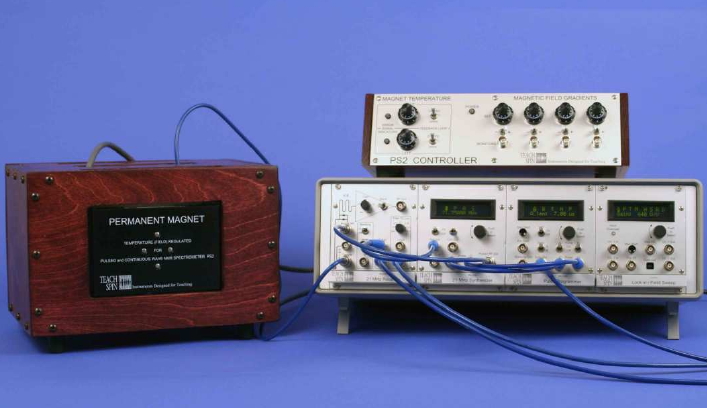
\includegraphics[scale=0.5]{versuchsaufbau.png} 
\caption{Messapparatur der Firma Teachspin.}
%Teachspin manual
\label{fig:aufbau}
\end{figure}

Zunächst werden einige Einstellungen am Gerät vorgenommen.
Die PID-Temperaturreglung wird eingeschaltet, damit das Magnetfeld zeitlich konstant bleibt. 
Das Gerät wird auf die Larmorfrequenz des Protons eingestellt.
Mit Hilfe einer Testspule wurde der Resonanzschwingkreis justiert.
Daraufhin wurde mit dem FID vom leichten Mineralöl das Magnetfeld justiert.
Anschließend wird anhand einer Probe die optimale Zeit für einen $\pi$-Puls bestimmt, 
indem man die Pulszeit sukzessive vergrößert, bis das FID-Signal minimal wird.
Der $\frac{\pi}{2}$-Puls ergibt sich durch halbieren der optimalen Zeit, welche für den $\pi$-Puls bestimmt wurde.

Mit diesen Einstellungen wird die erste Versuchsreihe durchgeführt.
Für die 7 Proben (leichtes Mineralöl, schweres Mineralöl, Wasser, 100\% Glycerin, 50\% Glycerin/50\% Wasser, 20\% Glycerin/80\% Wasser, 10\% Glycerin/90\% Wasser )
werden folgende Messreihen durchgeführt:
\begin{enumerate}[itemsep=0pt] 
\item Free Induction Decay (FID)
\item Spin Echo (SE) (mit 12 verschiedenen Pulsabständen)
\item Meiboom-Gill (MG) 
\item Inversion Recovery (IR) (mit 12 verschiedenen Pulsabständen)
\end{enumerate}

Zusätzlich wird nur für das leichte Mineralöl eine Carr-Purcell (CP) Sequenz aufgenommen.
Bei allen Messungen ist darauf zu achten, genügend große Periodendauern zu wählen, damit die Kerne relaxieren können, bevor die nächste Messung beginnt.

Für die Untersuchung der fluorinierten Probe wird die Apparatur auf deren Larmorfrequenz eingestellt. 
Es wird ein FID- Signal aufgenommen und fouriertransformiert.

\section{Auswertung}

Die Auswertung wird exemplarisch für die Probe \glqq leichtes Mineralöl\grqq~durchgeführt. Die Plots der anderen Proben befinden sich im Anhang. Die berechneten Relaxationszeiten aller Proben sind in Tabelle \ref{tab:relaxationszeiten} aufgelistet.

\subsection{Free Induction Decay}

Zunächst wird die induzierte Spannung nach einem $\frac{\pi}{2}$-Puls gemessen. Dieses Signal wird free induction decay genannt. Aus dem exponentiellen Abfall der induzierten Spannung lässt die Zeitkonstante $T_{2}^*$ bestimmen. Diese Zeit beinhaltet neben der Spin-Spin-Relaxationszeit, jedoch auch statische Dephasierungseffekte, hauptsächlich durch Inhomogenitäten des Magnetfeldes bedingt.
Die Zeitkonstante $T_{2}^*$ ist also größer als die tatsächliche Spin-Spin-Relaxationszeit.

An die Messdaten wird eine Funktion der Form
\begin{equation}
U_{\text{ind}}(t)=U_0 \exp(-t/T_{2}^*) + U_{\text{off}}
\end{equation}
gefittet (Abbildung \ref{fig:FID}).
Mit Matlab ergeben sich folgende Fitparameter:
\begin{align*} 
U_0 	&\approx  \SI{3,391(7)}{\volt} \\ 
T_{2}^{\text{*}} &\approx  \SI{4,501(7)}{\milli\second} \\
U_{\text{off}}	&\approx  \SI{0,1249(2)}{\volt}{.}
\end{align*}

\begin{figure}[H]
\centering
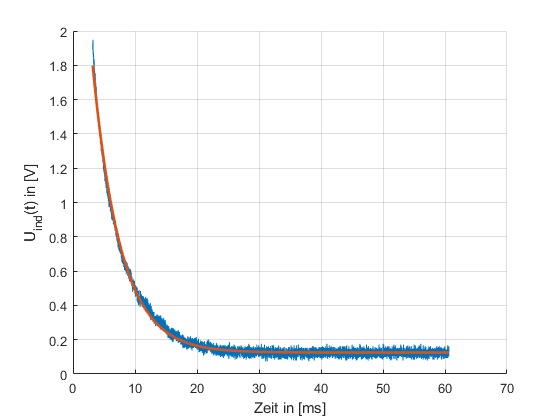
\includegraphics[scale=0.6]{FID/FIDleichtesMineral.png} 
\caption{FID Messung für leichtes Mineralöl.}
\label{fig:FID}
\end{figure}
\newpage
\subsection{Spin-Echo}

Um die Spin-Spin-Relaxationzeit, die nur von stochastischen Dephasierungsprozessen abhängt, genauer zu messen, wird eine Spin Echo Messung durchgeführt.
Bei dieser wird nach dem $\frac{\pi}{2}$-Puls nach einer variablen Wartezeit $\tau$ ein $\pi$-Puls eingestrahlt. Das hat zur Folge, dass sich statische Dephasierungsprozesse kompensieren. Die Magnetisierung erreicht nach der Zeit $t=2\,\tau$ ein Maximum (Echo).
Misst man für verschiedene $\tau$ das Maximum, und passt eine Exponentialfunktion an diese an, wie bei der Messung des FID Signals, so erhält man eine größere und genauere Spin-Spin-Relaxationzeit, als bei der ersten Messung.

An die Messdaten wird eine Funktion der Form
\begin{equation}
U_{\text{ind}}(t)= U_0 \exp(-t/T_{2}^{CP}) + U_{\text{off}}
\end{equation}
gefittet (Abbildung \ref{fig:SE}).
Es ergeben sich folgende Fitparameter:
\begin{align*} 
U_0 	&\approx  \SI{7,524(456)}{\volt} \\ 
T_{2}^{SE} &\approx  \SI{47,19(473)}{\milli\second} \\
U_{\text{off}}	&\approx  \SI{0,2934(1172)}{\volt}
\end{align*}

\begin{figure}[H]
\centering
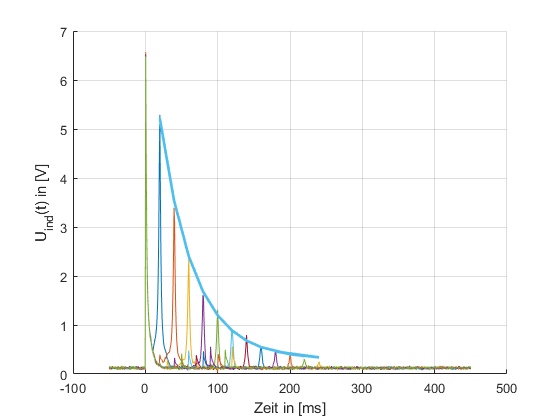
\includegraphics[scale=0.6]{Echo/leichtemineralol/Plot.png}
\caption{Spin Echo Messung für leichtes Mineralöl. Durch die Maxima wird eine Exponentialfunktion gelegt.}
\label{fig:SE}
\end{figure}

\subsection{Carr-Purcell und Meiboom-Gill}

Die Carr-Purcell-Methode funktioniert prinzipiell wie die Spin-Echo-Methode. Die Messungen für verschiedene $\tau$ werden jetzt automatisch mit einer Pulssequenz durchgeführt. Die Sequenz besteht aus einem $\frac{\pi}{2}$-Puls, gefolgt von mehreren $\pi$-Pulsen zu den Zeiten $\tau$, 3$\tau$, 5$\tau$, ... . Jeweils zwischen 2 $\pi$-Pulsen liegt ein Echo. Die Echos fallen exponentiell mit der Zeit ab. Passt man eine Funktion der Form
\begin{equation}
U_{\text{ind}}(t)=U_0 \exp(-t/T_{2}^{CP}) + U_{\text{off}}
\end{equation}
an die Maxima an (Abbildung \ref{fig:CP}), so ergeben sich die Parameter:
\begin{align*} 
U_0 	&\approx  \SI{6,923(129)}{\volt} \\ 
T_{2}^{CP} &\approx  \SI{59,7(30)}{\milli\second} \\
U_{\text{off}}	&\approx  \SI{0,2887(970)}{\volt} 
\end{align*}
Die Carr-Purcell-Methode hat jedoch einen großen Nachteil. Da der $\pi$-Puls nicht exakt eingestellt werden kann, summieren sich hier die Fehler auf. Ist der Puls ein bisschen zu lang oder zu kurz, wird die Magnetisierung nicht genau in die Messebene geklappt. Er hat dann auch eine Komponente in Magnetfeldrichtung. Diese Komponente wird nach jedem $\pi$-Puls größer, ist jedoch nicht messbar.
Auch die hier gemessene Zeitkonstante $T_2^{CP}$ ist also kleiner als die Spin-Spin-Relaxationzeit.

Um dieses neue Problem zu umgehen, nutzt man die Meiboom-Gill-Methode.
Sie besteht aus der gleichen Pulssequenz wie die CP-Methode, jedoch sind die $\pi$-Pulse gegenseitig phasenverschoben. 
Dadurch hebt sich ein Fehler in der Pulslänge nach jedem zweiten Durchgang auf.
Die Meiboom-Gill-Methode ist von den betrachteten Methoden die genaueste zur Bestimmung der Spin-Spin-Relaxationzeit.
Auch an diese Messreihe wird eine Exponentialfunktion angepasst. Es ergeben sich die Parameter:
\begin{equation}
U_{\text{ind}}(t)=U_0 \exp(-t/T_{2}^{MG}) + U_{\text{off}}{.}
\end{equation}
Passt man eine Funktion an die Maxima an (Abbildung \ref{fig:MG}), so ergeben sich die Parameter:
\begin{align*} 
U_0 	&\approx  \SI{6,702(195)}{\volt} \\ 
T_{2}^{MG} &\approx  \SI{53,75(382)}{\milli\second} \\
U_{\text{off}}	&\approx  \SI{0,435(1089)}{\volt} 
\end{align*}
\begin{figure}[H]
\centering
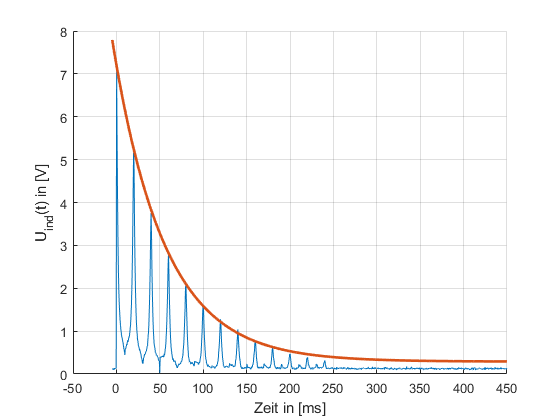
\includegraphics[scale=0.6]{CP/leichtesmineral.png} 
\caption{CP Messung für leichtes Mineralöl. Durch die Maxima wird eine Exponentialfunktion gelegt.}
\label{fig:CP}
\end{figure}
\newpage
\begin{figure}[H]
\centering
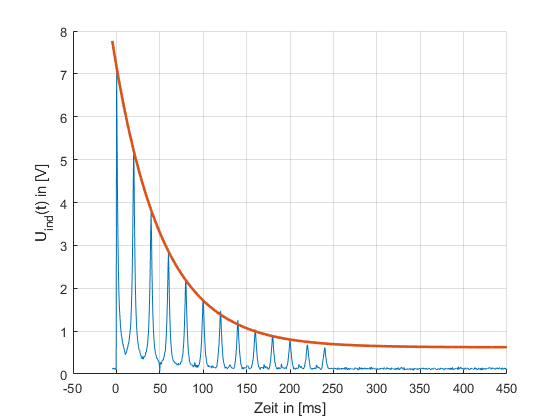
\includegraphics[scale=0.6]{MG/leichtesmineral.png} 
\caption{MG Messung für leichtes Mineralöl. Durch die Maxima wird eine Exponentialfunktion gelegt.}
\label{fig:MG}
\end{figure}
\newpage
\subsection{Inversion Recovery}

Nach der Ermittlung der Spin-Spin-Relaxationzeit wird jetzt die Spin-Gitter-Relaxationzeit der Proben bestimmt.
Dazu strahlt man einen $\pi$-Puls auf die Probe, gefolgt, nach einer Wartezeit von 2 $\tau$, von einem $\frac{\pi}{2}$-Puls.
Durch den $\frac{\pi}{2}$-Puls wird das Vorzeichen der Magnetisierung umgekehrt. Die Magnetisierung relaxiert dadurch exponentiell zurück in den Gleichgewichtszustand. Da die Magnetisierung in Magnetfeldrichtung jedoch nicht messbar ist, wird nach verschieden langen Wartezeiten ein $\pi$-Puls eingestrahlt. Dadurch wird die Magnetisierung in die Messebene geklappt. Das gemessene Maximum entspricht der Magnetisierung in Magnetfeldrichtung.
Legt man eine Kurve der Form:
\begin{equation}
U_{\text{ind}}(t)=U_0 \left( 1- 2 \exp(-t/T_{1}^{IR}) \right) + U_{\text{off}}
\end{equation}
durch die Maxima (Abbildung 6), ergeben sich folgende Parameter:
\begin{align*} 
U_0 	&\approx  \SI{6,697(105)}{\volt} \\ 
T_{2}^{MG} &\approx  \SI{59,61(332)}{\milli\second} \\
U_{\text{off}}	&\approx  \SI{-1,126(220)}{\volt} 
\end{align*}\par

\begin{figure}[H]
\centering
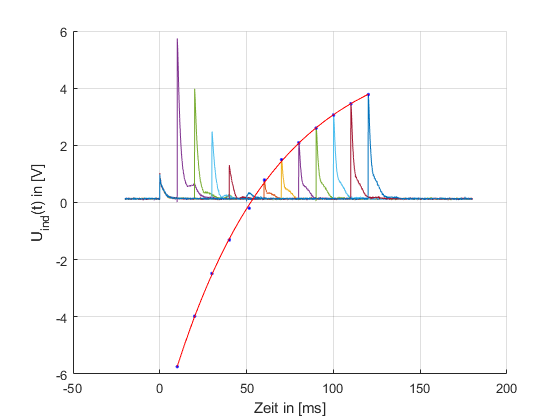
\includegraphics[scale=0.7]{IR/leichtesmineral/Plot.png} 
\caption{IR Messung für leichtes Mineralöl. Durch die Maxima wird eine Exponentialfunktion gelegt.}

\end{figure}
\newpage
\subsection{Berechnete Relaxationszeiten aller Proben}

Die berechneten Relaxationszeiten aller Proben sind in Tabelle \ref{tab:relaxationszeiten} aufgelistet.

Wie erwartet, klingt das FID Signal aller Proben sehr schnell ab. Die Zeitkonstante $T_2^*$ liegt im Bereich von 1,3 - 4,5 ms.

Die aus den SE Messungen bestimmten Relaxationszeiten sind länger als das FID Signal, noch länger sind die aus den MG Messungen, außer beim schweren Mineralöl. Beide Zeiten liegen jedoch relativ nah beieinander, und überschneiden sich innerhalb der Toleranzgrenzen.

Die aus der CP Methode bestimmte Zeit, ist, wider der Erwartung, etwas länger als die aus der MG Messung bestimmten Zeit. Innerhalb der Toleranzgrenzen überschneiden sich die Werte. 

Die Messungen der Proben mit einem unterschiedlichen Mischungsverhältnis aus Glycerin und Wasser, sind überwiegend konsistent. Je höher der Anteil an Glycerin, desto kleiner wird die Relaxationszeit. Ausreißer sind jedoch die berechnete Spin-Gitter-Relaxationszeit von Wasser mit 778 ms, die kleiner ist als die der Glycerin-Wasser-Lösungen.
Beim SE-Versuch ist ebenfalls die 50\%-ige Lösung größer als die 20\%-ige, und beim IR Versuch die 20\%-ige größer als die 10\%-ige.

Die berechneten Relaxationszeiten von Wasser weichen stark ab von den gefundenen Literaturwerten (Quellenverweis). Es liegt wahrscheinlich ein grober systematischer Messfehler vor. Eine Vermutung ist, dass die Periodenlänge zu kurz eingestellt war.

Die Messungen für die Öle scheinen genauer zu sein, ein Vergleich mit Literaturwerten zeigt, dass diese in der selben Größenordnung liegen. (Quellenverweis)

Vergleicht man die Zeiten von Glycerin mit den Literaturwerten (Quellenvwerweis), fällt auf, dass beide Relaxationszeiten mit allen Methoden zu lang bestimmt werden.

\begin{landscape}
\begin{table}[H]
\centering
\caption{Aus dem Fit gewonnene Relaxationszeiten der Proben mit den unterschiedlichen Messmethoden. Zum Vergleich stehen die bekannten Literaturwerte (Quellenverweis) in den letzten zwei Spalten.}
\begin{tabular}{lllllll}
		\hline
       & FID          & SE          & MG          & IR          & Literatur   & Literatur   \\ 
       & $T_2^*$ in ms& $T_2^{SE}$ in ms	& $T_2^{MG}$ in ms	& $T_1^{IR}$ in ms	& $T_1$ in ms	& $T_2$ in ms	\\
       \hline
Wasser & 2,057 $ \pm $ 0,008 & 596,4 $\pm$ 955,6 & 777,6 $\pm$ 112,1 & 778,5 $\pm$ 1286,5 & 3518,00 & 2000,00 \\
10\% Glycerin   & 1,626 $\pm$ 0,006 & 201,6 $\pm$ 52,7  & 420,9 $\pm$ 118,9 & 1763 $\pm$ 2122 & - & - \\
20\%  Glycerin & 1,36 $\pm$ 0,003  & 144,4 $\pm$ 16,1  & 308,5 $\pm$ 70,6  & 1948 $\pm$ 1881  & - & - \\
50\% Glycerin  & 2,33 $\pm$ 0,008  & 169,8 $\pm$ 22,5  & 269,2 $\pm$ 68,0  & 1590 $\pm$ 811  & - & - \\
Glycerin  & 2,247 $\pm$ 0,005 & 87,65 $\pm$ 6,15  & 112,8 $\pm$ 10,50 & 346,3 $\pm$ 272 & 41,00 & 43,5 \\
leichtes Öl & 4,501 $\pm$ 0,007 & 47,19 $\pm$ 4,73  & 53,75 $\pm$ 3,82  & 59,61 $\pm$ 3,32  & 52,216 & 64,027 \\
schweres Öl & 1,563 $\pm$ 0,004 & 24,32 $\pm$ 0,9   & 22,04 $\pm$ 1,5   & 31,19 $\pm$ 1,9  & 34,388 & 31,546 \\
\hline
\label{tab:relaxationszeiten}
\end{tabular}
\end{table}

Die berechnete Spin-Spin-Relaxationszeit von leichtem Mineralöl nach der CP-Methode beträgt: $T_{2}^{CP} \approx  \SI{59,7(30)}{\milli\second} $

\end{landscape}

\subsection{Fluorinert Probe}

Für die fluorinerte Probe wird das FID-Signal gemessen, und anschließend fouriertransformiert.
\begin{figure}[H]
\centering
\begin{subfigure}{.4\textwidth}
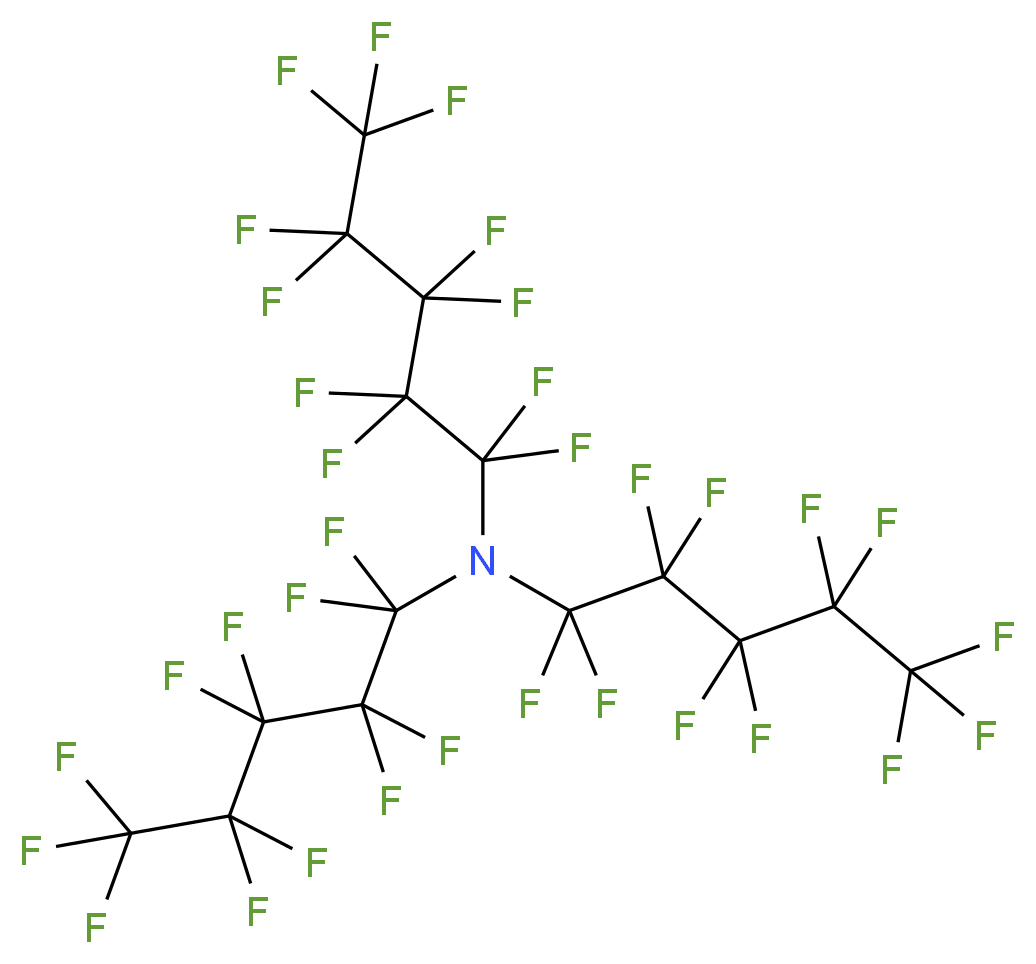
\includegraphics[scale=0.15]{fluorinert.png} 
\caption{Strukturformel von Fluorinert FC-70.}
%%http://en.chembase.cn/substance-181368.html#2d_img
\label{fig:fluorinert}
\end{subfigure} %
\begin{subfigure}{.59\textwidth}
\centering
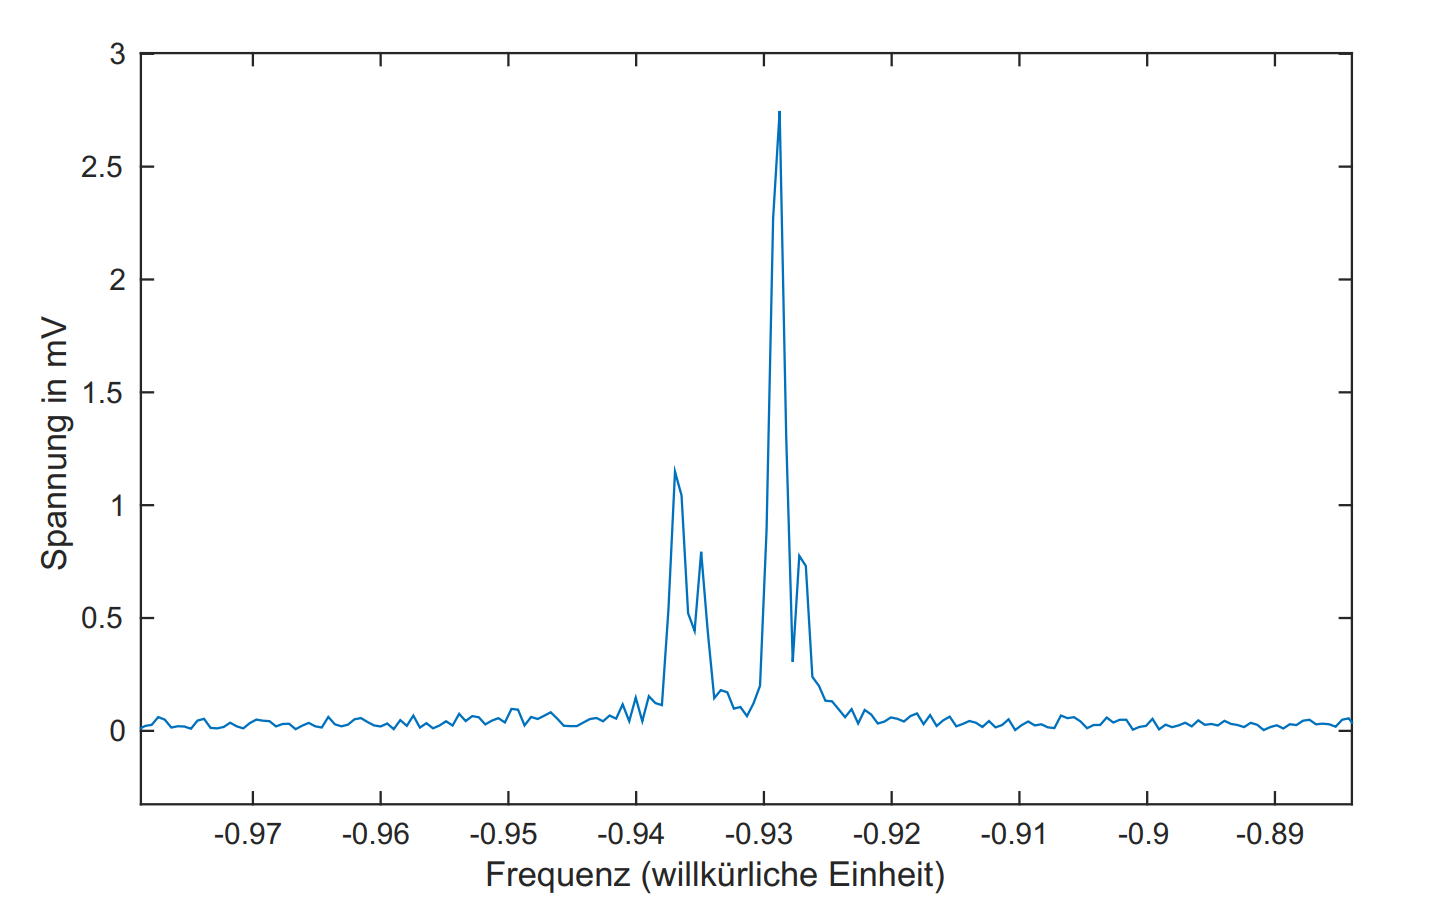
\includegraphics[scale=0.35]{fft_fluorinert2.PNG} 
\caption{Fouriertransformierte des FID-Signals der fluorinerten Probe.}
\label{fig:fft}
\end{subfigure}
\end{figure}

Das Frequenzspektrum zeigt deutlich vier relativ nahe beieinander liegende Peaks (Abbildung \ref{fig:fft}).
Das Signal stammt von den Fluor-Kernen.
Abbildung \ref{fig:fluorinert} zeigt die Struktur des betrachteten Moleküls Fluorinert FC-70. Man erkennt, dass die Fluor-Atome im Molekül sich in unterschiedlichen Umgebungen befinden. Sie befinden sich dadurch auch in unterschiedlichen lokalen Magnetfeldern. Daher haben sie auch leicht verschiedene Resonanzfrequenzen.

\section{Fehlerbetrachtung}

Den groben Ausreißern liegen vermutlich systematische Fehler zugrunde. Möglich ist, dass die Probe nicht richtig in den Messapparat eingesetzt wurde, oder, dass die Periodenlänge nicht lang genug gewählt wurde. Auch im Messprogramm liegen mögliche Fehlerquellen, es kam vor, dass das Programm die Werte nicht aktualisierte, oder einen unangepassten Wertebereich anzeigte.

\section{Zusammenfassung}

Insgesamt betrachtet sind die Messungen für Wasser, Glycerin und die Glycerinlösungen relativ ungenau im Vergleich zu den gefunden Literaturwerten, es lässt sich jedoch eine Tendenz erkennen.

Die Messungen der Öle scheint genauer zu sein und ein Vergleich mit Literaturwerten (Quellenvwerweis) zeigt, dass diese in der selben Größenordnung liegen.

Wie erwartet, klingt das FID-Signal aller Proben sehr schnell ab. Die Zeitkonstante $T_2^*$ liegt im Bereich von 1,3 - 4,5 ms.

Die aus den SE Messungen bestimmten Relaxationszeiten sind länger als die Zeitkonstanten des FID-Signals und sind noch länger als aus den MG-Messungen, außer beim schweren Mineralöl.

Die aus der CP-Methode bestimmte Zeit, ist, wider der Erwartung, länger als die aus der MG-Messung bestimmten Zeit.

Die Messungen der Proben mit einem unterschiedlichen Mischungsverhältnis aus Glycerin und Wasser, sind überwiegend konsistent. Je höher der Anteil an Glycerin, desto kleiner wird die Relaxationszeit.

Die vier Peaks im fouriertransformierten FID-Signal der Fluor- Probe zeigen qualitativ, dass Fluoratome in verschiedenen Bindungspositionen vorliegen.



\section{Anhang}
\subsection{Free Induction Decay}
\begin{figure}[H]
\centering
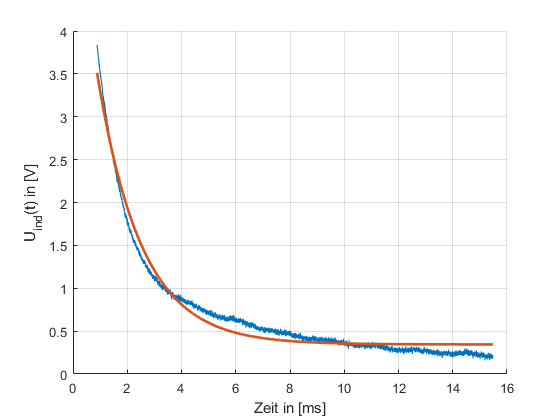
\includegraphics[scale=0.75]{FID/FID10Glycerin.png} 
\caption{Free Induction Decay von einer Lösung aus 10\% Glycerin und 90\% Wasser mit einer exponentiellen Fitfunktion.}
\end{figure}
\begin{figure}[H]
\centering
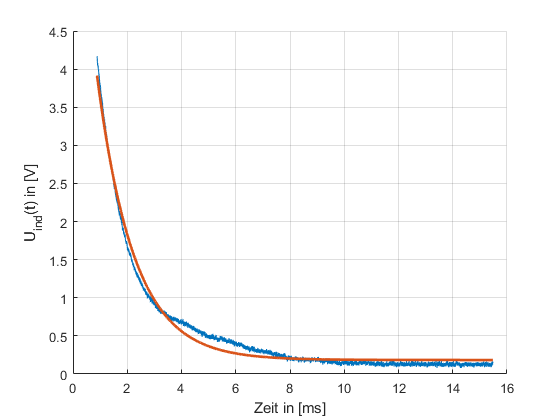
\includegraphics[scale=0.75]{FID/FID20Glycerin.png} 
\caption{Free Induction Decay von einer Lösung aus 20\% Glycerin und 80\% Wasser mit einer exponentiellen Fitfunktion.}
\end{figure}
\begin{figure}[H]
\centering
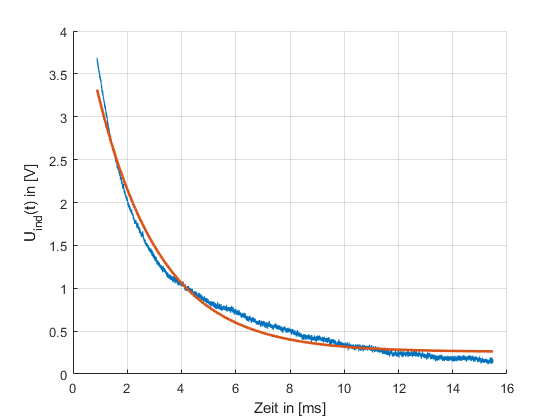
\includegraphics[scale=0.75]{FID/FID50Glycerin.png} 
\caption{Free Induction Decay von einer Lösung aus 50\% Glycerin und 50\% Wasser mit einer exponentiellen Fitfunktion.}
\end{figure}
\begin{figure}[H]
\centering
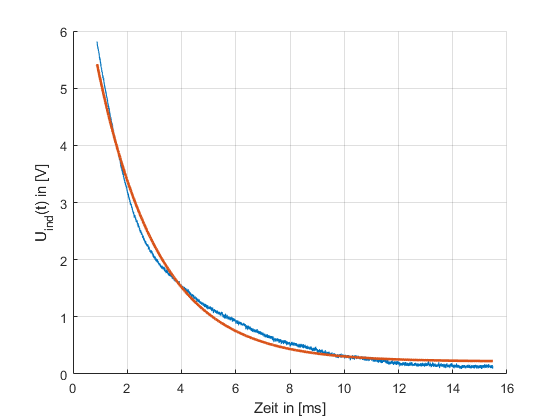
\includegraphics[scale=0.75]{FID/FID100Glycerin.png} 
\caption{Free Induction Decay der Glycerin Probe mit einer exponentiellen Fitfunktion.}
\end{figure}
\begin{figure}[H]
\centering
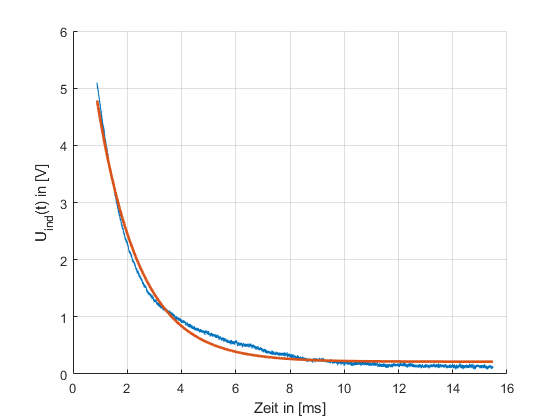
\includegraphics[scale=0.75]{FID/FIDschweresMineral.png} 
\caption{Free Induction Decay der schweren Mineralöl Probe mit einer exponentiellen Fitfunktion.}
\end{figure}
\begin{figure}[H]
\centering
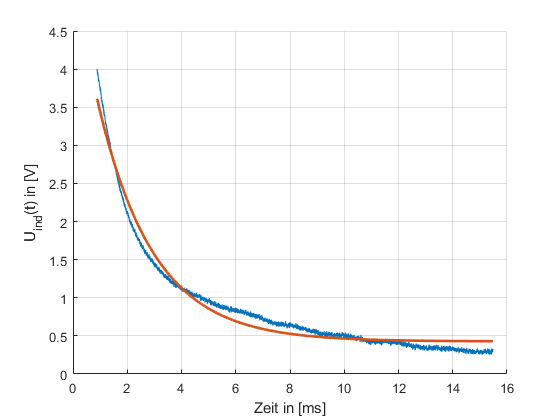
\includegraphics[scale=0.75]{FID/FIDWasser.png} 
\caption{Free Induction Decay von Wasser mit einer exponentiellen Fitfunktion.}
\end{figure}
\subsection{Spin Echo}
\begin{figure}[H]
\centering
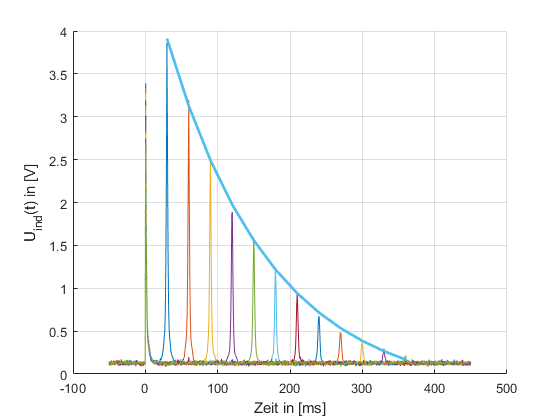
\includegraphics[scale=0.75]{Echo/10Glycerin/Plot.png} 
\caption{Spin Echo Messung für eine Lösung aus 10\% Glycerin und 90\% Wasser. Durch die Maxima wird eine Exponentialfunktion gelegt.}
\end{figure}
\begin{figure}[H]
\centering
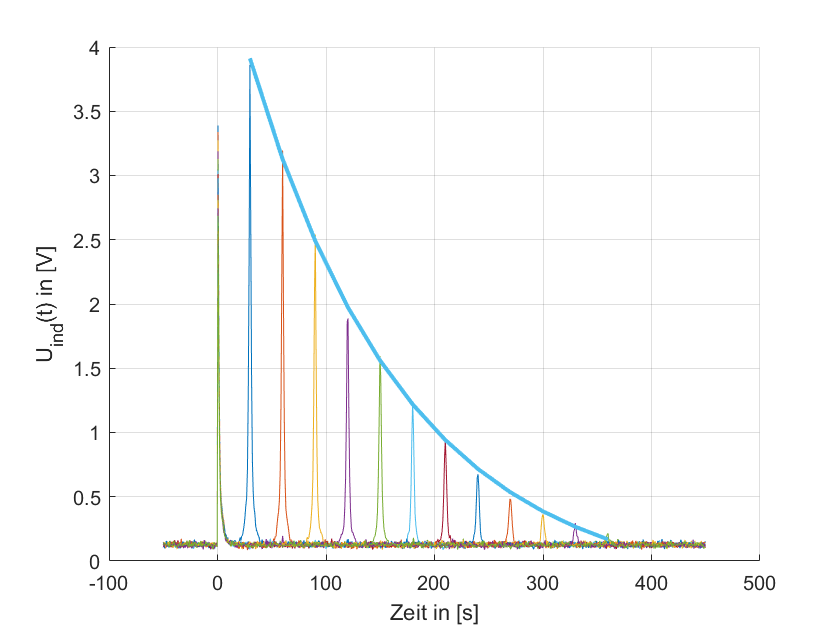
\includegraphics[scale=0.45]{Echo/20Glycerin/Plot.png} 
\caption{Spin Echo Messung für eine Lösung aus 20\% Glycerin und 80\% Wasser. Durch die Maxima wird eine Exponentialfunktion gelegt.}
\end{figure}
\begin{figure}[H]
\centering
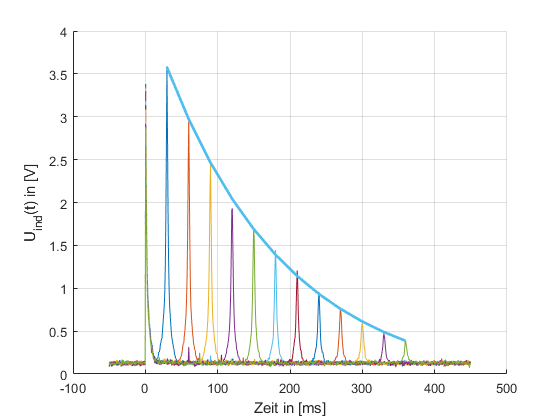
\includegraphics[scale=0.75]{Echo/50Glycerin/Plot.png} 
\caption{Spin Echo Messung für eine Lösung aus 50\% Glycerin und 50\% Wasser. Durch die Maxima wird eine Exponentialfunktion gelegt.}
\end{figure}
\begin{figure}[H]
\centering
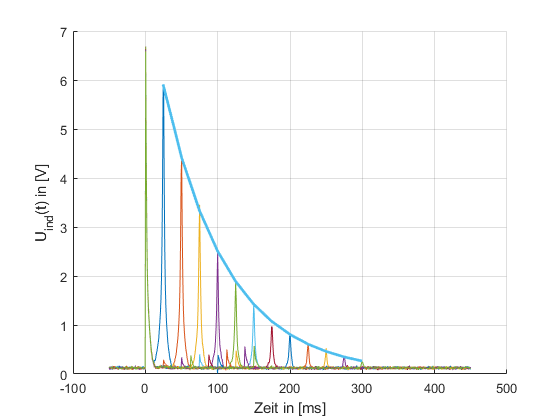
\includegraphics[scale=0.75]{Echo/Glycerin/Plot.png} 
\caption{Spin Echo Messung für Glycerin. Durch die Maxima wird eine Exponentialfunktion gelegt.}
\end{figure}
\begin{figure}[H]
\centering
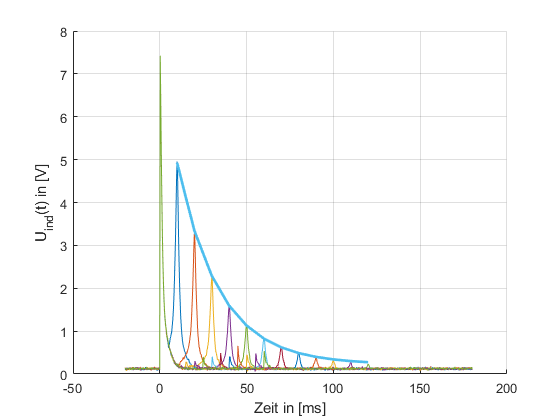
\includegraphics[scale=0.75]{Echo/schweresmineralol/Plot.png} 
\caption{Spin Echo Messung für schweres Mineralöl. Durch die Maxima wird eine Exponentialfunktion gelegt.}
\end{figure}
\begin{figure}[H]
\centering
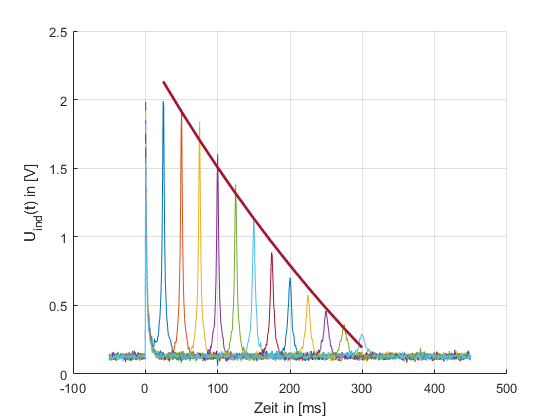
\includegraphics[scale=0.75]{Echo/Wasser/Plot.png} 
\caption{Spin Echo Messung für Wasser. Durch die Maxima wird eine Exponentialfunktion gelegt.}
\end{figure}
\subsection{Meiboom-Gill}
\begin{figure}[H]
\centering
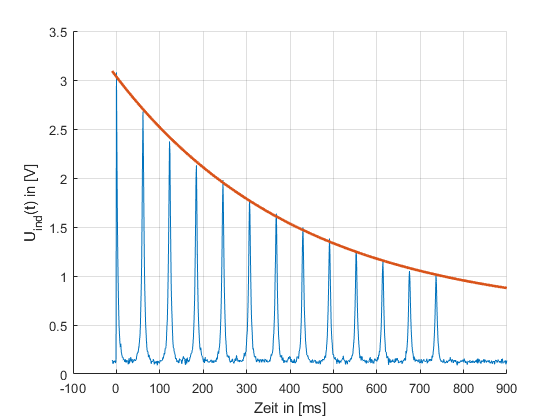
\includegraphics[scale=0.75]{MG/10Glycerin.png} 
\caption{Meiboom-Gill Messung für eine Lösung aus 10\% Glycerin und 90\% Wasser. Durch die Maxima wird eine Exponentialfunktion gelegt.}
\end{figure}
\begin{figure}[H]
\centering
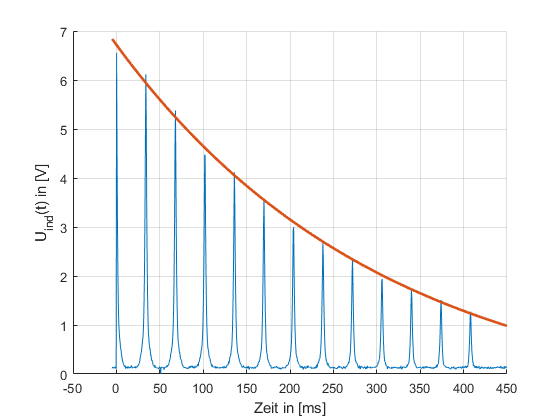
\includegraphics[scale=0.65]{MG/20Glycerin.png} 
\caption{Meiboom-Gill Messung für eine Lösung aus 20\% Glycerin und 80\% Wasser. Durch die Maxima wird eine Exponentialfunktion gelegt.}
\end{figure}
\begin{figure}[H]
\centering
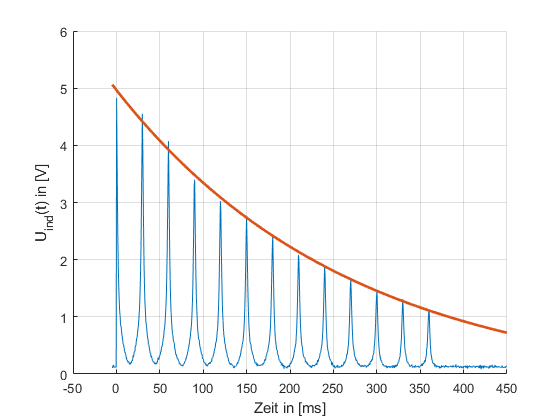
\includegraphics[scale=0.65]{MG/50Glycerin.png} 
\caption{Meiboom-Gill Messung für eine Lösung aus 50\% Glycerin und 50\% Wasser. Durch die Maxima wird eine Exponentialfunktion gelegt.}
\end{figure}
\begin{figure}[H]
\centering
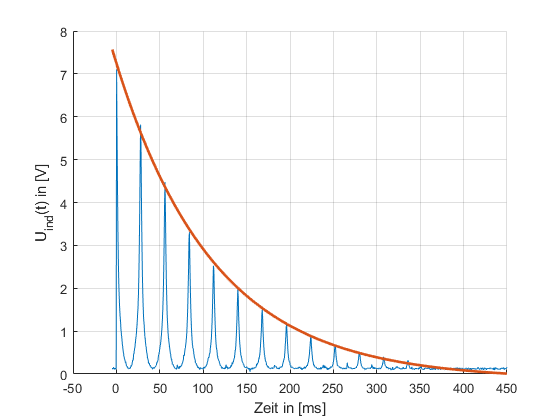
\includegraphics[scale=0.65]{MG/100Glycerin.png} 
\caption{Meiboom-Gill Messung für Glycerin. Durch die Maxima wird eine Exponentialfunktion gelegt.}
\end{figure}
\begin{figure}[H]
\centering
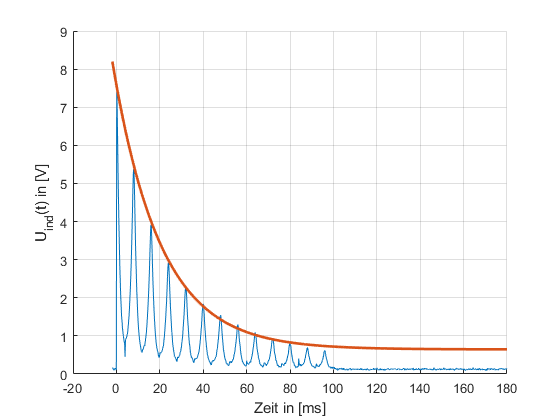
\includegraphics[scale=0.65]{MG/schweresMineral.png} 
\caption{Meiboom-Gill Messung für schweres Mineralöl. Durch die Maxima wird eine Exponentialfunktion gelegt.}
\end{figure}
\begin{figure}[H]
\centering
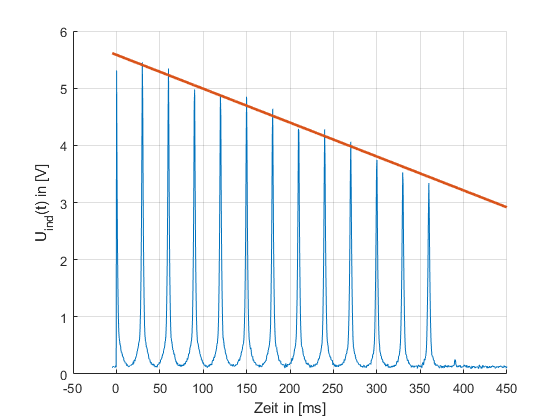
\includegraphics[scale=0.65]{MG/Wasser.png} 
\caption{Meiboom-Gill Messung für Wasser. Durch die Maxima wird eine Exponentialfunktion gelegt.}
\end{figure}
\subsection{Inversion Recovery}
\begin{figure}[H]
\centering
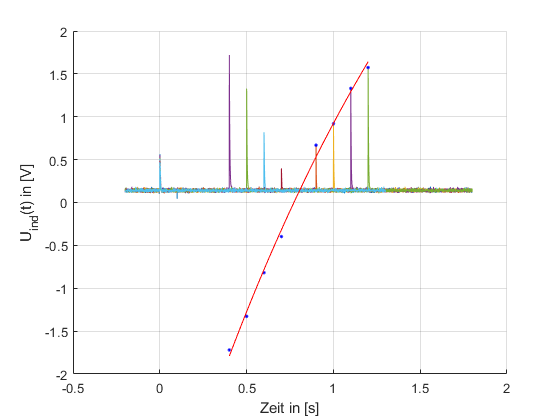
\includegraphics[scale=0.7]{IR/10Glycerin/Plot.png} 
\caption{Inversion Recovery Messung für eine Lösung aus 10\% Glycerin und 90\% Wasser. Durch die Maxima wird eine Exponentialfunktion gelegt.}
\end{figure}
\begin{figure}[H]
\centering
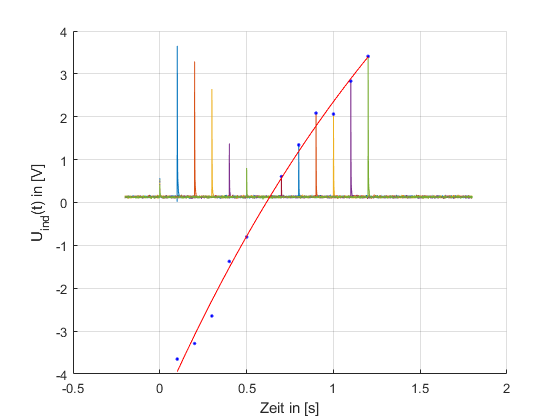
\includegraphics[scale=0.7]{IR/20Glycerin/Plot.png} 
\caption{Inversion Recovery Messung für eine Lösung aus 20\% Glycerin und 80\% Wasser. Durch die Maxima wird eine Exponentialfunktion gelegt.}
\end{figure}
\begin{figure}[H]
\centering
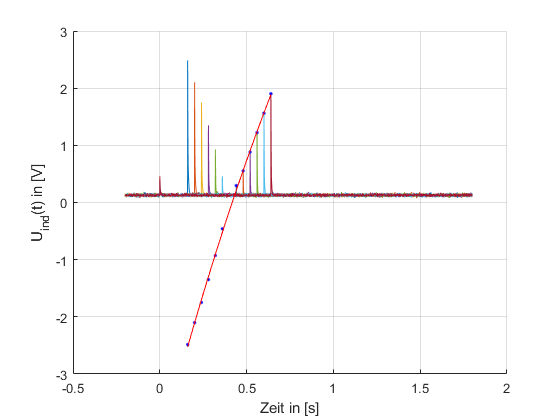
\includegraphics[scale=0.7]{IR/50Glycerin/Plot.png} 
\caption{Inversion Recovery Messung für eine Lösung aus 50\% Glycerin und 50\% Wasser. Durch die Maxima wird eine Exponentialfunktion gelegt.}
\end{figure}
\begin{figure}[H]
\centering
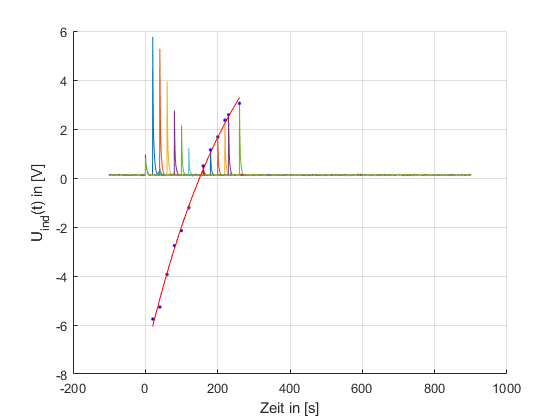
\includegraphics[scale=0.7]{IR/Glycerin/Plot.png} 
\caption{Inversion Recovery Messung für Glycerin. Durch die Maxima wird eine Exponentialfunktion gelegt.}
\end{figure}
\begin{figure}[H]
\centering
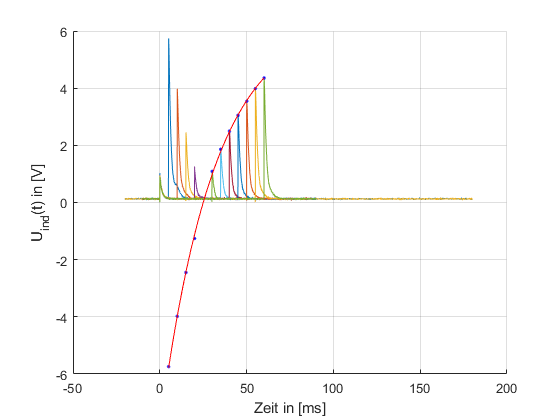
\includegraphics[scale=0.7]{IR/schweresmineral/Plot.png} 
\caption{Inversion Recovery Messung für schweres Mineralöl. Durch die Maxima wird eine Exponentialfunktion gelegt.}
\end{figure}
\begin{figure}[H]
\centering
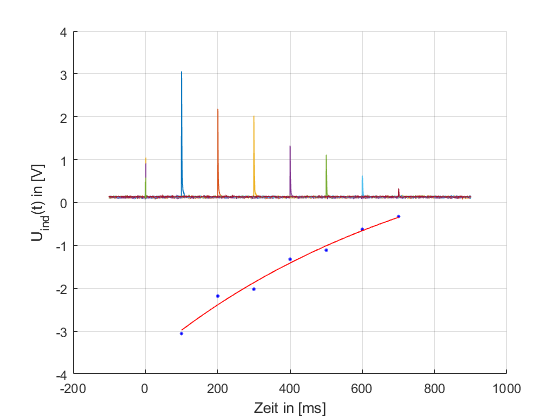
\includegraphics[scale=0.7]{IR/Wassser/Plot.png} 
\caption{Inversion Recovery Messung für Wasser. Durch die Maxima wird eine Exponentialfunktion gelegt.}
\end{figure}

%Literaturwerte
%http://home.sandiego.edu/~severn/p480w/pnm_jc_draft2.pdf Glycerin Mineralöl
%http://mri-q.com/why-is-t1--t2.html Wasser
%https://neurophysics.ucsd.edu/courses/physics_173_273/pulsed_NMR_heme.pdf Glycerin 17/18

\renewcommand{\refname}{\textbf{Literaturverzeichnis}}
\begin{thebibliography}{xx}

 		  \bibitem[1]{1}		
\glqq Literaturwerte Glycerin und Mineralöl\grqq ,\\
http://home.sandiego.edu/$\sim$severn/p480w/pnm\_jc\_draft2.pdf , 
 	31.Mai.2018
    	 \bibitem[2]{2}			
\glqq Literaturwerte Wasser\grqq ,
http://mri-q.com/why-is-t1--t2.html,
31.Mai.2018
   		 \bibitem[3]{3}			
\glqq Glycerin 17/18\grqq ,\\
https://neurophysics.ucsd.edu/courses/physics\_173\_273/pulsed\_NMR\_heme.pdf,
31.Mai.2018 
\end{thebibliography}

Für die Theorie wurden die Versuchsanleitung und das Experimetalphysik5-Skript, Wintersemester 2017/18, von Herrn Denninger verwendet.
Beide sind online nicht verfügbar, werden hier daher explizit nochmal erwähnt und können bei Bedarf nachgereicht werden.

\end{document}